Notre étude ce porteras dans un premier temps à vérifier que notre implémentation de LBM concorde avec la théorie.
Pour cela nous allons étudier l'écoulement de Poiseuille nous allons donc placer un profil en forme de tube dans notre simulation. Pour vérifier la corrélation avec les résultats théorique nous allons intégrer le débit volumique à deux
niveau et on vas pouvoir ainsi vérifier la conservation du débit volumique.
En plus nous avons la formule théorique de l'écoulement de Poiseuille 

\begin{equation}
  v(z) = v_\text{max} \left(\frac{4z}{h} - \frac{4z^2}{h^2}\right),
\end{equation}

en intégrant sur $h$ on obtiens $v_\text{max}$ en fonction du débit volumique $D_v$ : 

\begin{equation}
  D_v = v_\text{max} \frac{2h}{3}.
\end{equation}

Étant donné que notre écoulement et incompressible en intégrant numériquement sur une première section on obtiens donc 
le profil de vitesse pour la deuxième section :

\begin{equation}
  v(x) = D_v \frac{3}{2h} \left( \frac{4z}{h} - \frac{4z^2}{h^2} \right).
\end{equation}

Voici les différents résultats obtenus :

\begin{figure}[hbtp]
  \centering
  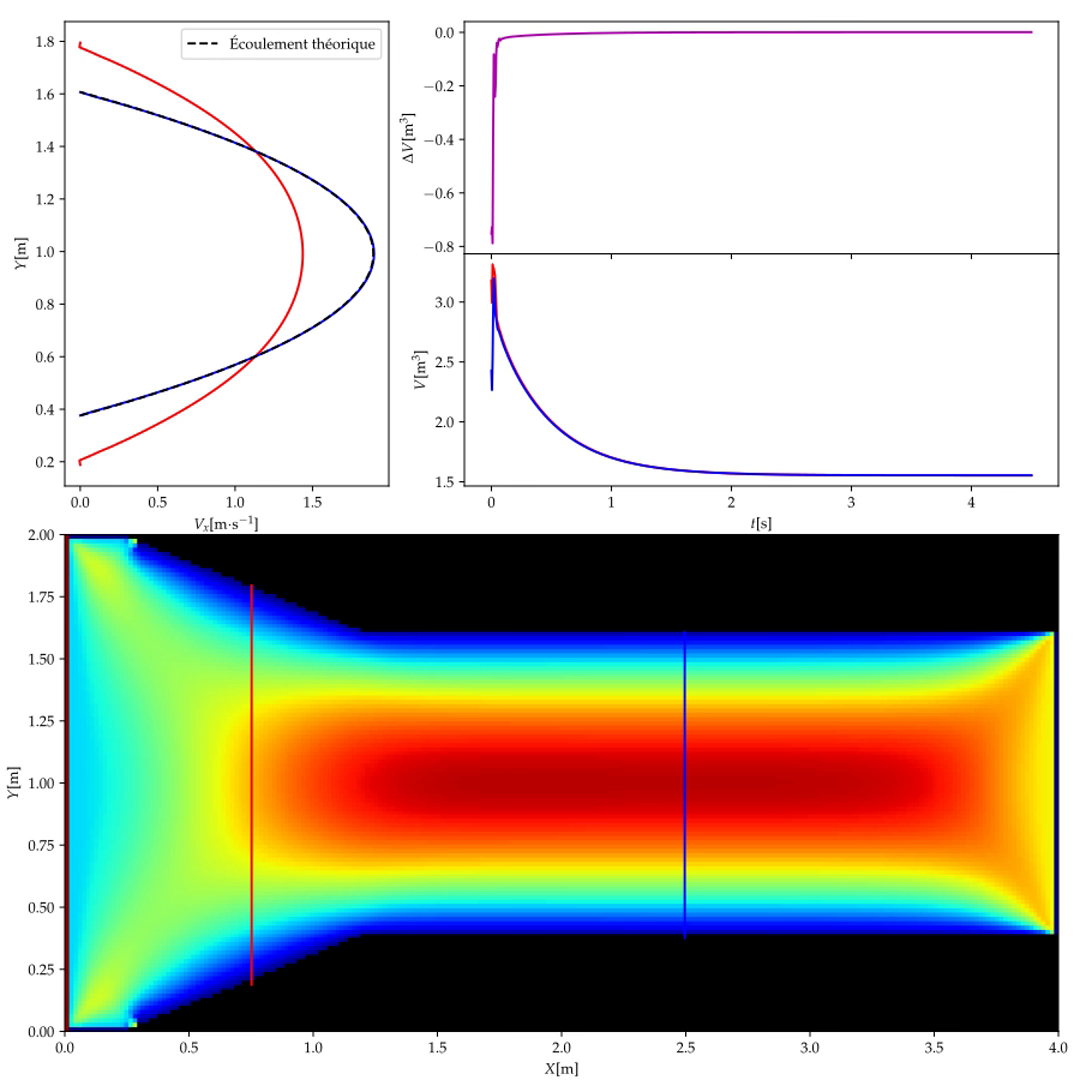
\includegraphics[width=\linewidth]{Fig/Poiseuille.png}
  \caption{Étude de l'écoulement de Poiseuille dans un cas simple}
  \label{fig:P1}
\end{figure}
On observe que le débit volumique et conservée (à l'équilibre) de plus le profil des vitesse simulé colle parfaitement 
à la théorie. 
\begin{figure}[hbtp]
  \centering
  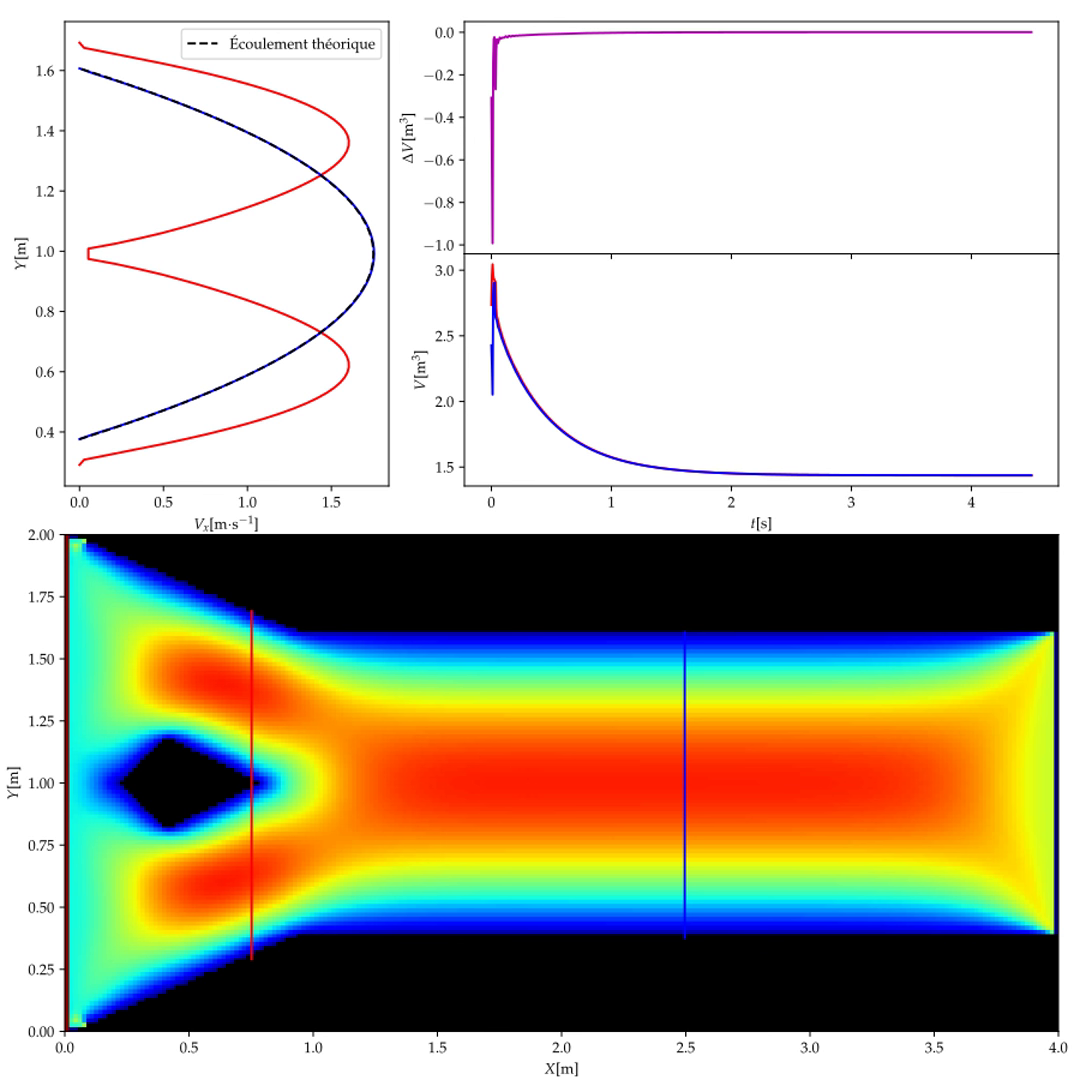
\includegraphics[width=\linewidth]{Fig/Poiseuille2.png}
  \caption{Étude de l'écoulement de Poiseuille dans une géométrie plus complexe}
  \label{fig:P2}
\end{figure}
\begin{figure}[hbtp]
  \centering
  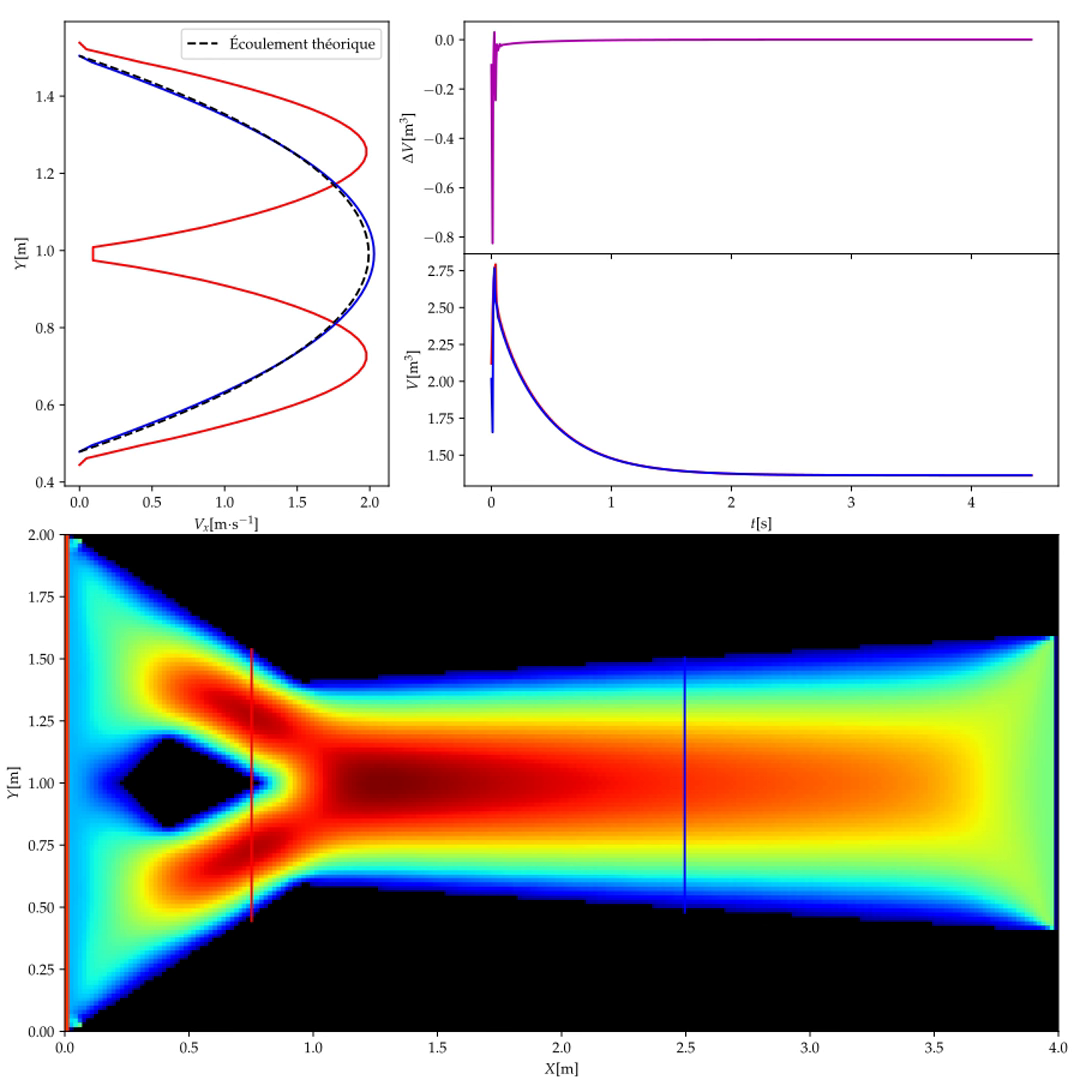
\includegraphics[width=\linewidth]{Fig/Poiseuille3.png}
  \caption{Étude de l'écoulement de Poiseuille dans une géométrie encore un peu plus complexe}
  \label{fig:P3}
\end{figure}

On observe pour la figure \ref{fig:P2} une nouvelle fois un très bon accord avec la théorie le débit volumique est toujours conservé. À partir de la figure \ref{fig:P3} le profil des vitesses ne colle plus totalement à la théorie, rien de très inquiétant étant donné que ce profile sort du domaine de définition de la théorie de poiseuille néanmoins le débit volumique et toujours conservé. 

Maintenant que nous avons confirmé que notre simulation concordais avec la théorie, nous pouvons essayer de simuler des 
systèmes non solvables analytiquement comme pour la figure \ref{fig:CF}. 

\begin{figure}[hbtp]
  \centering
  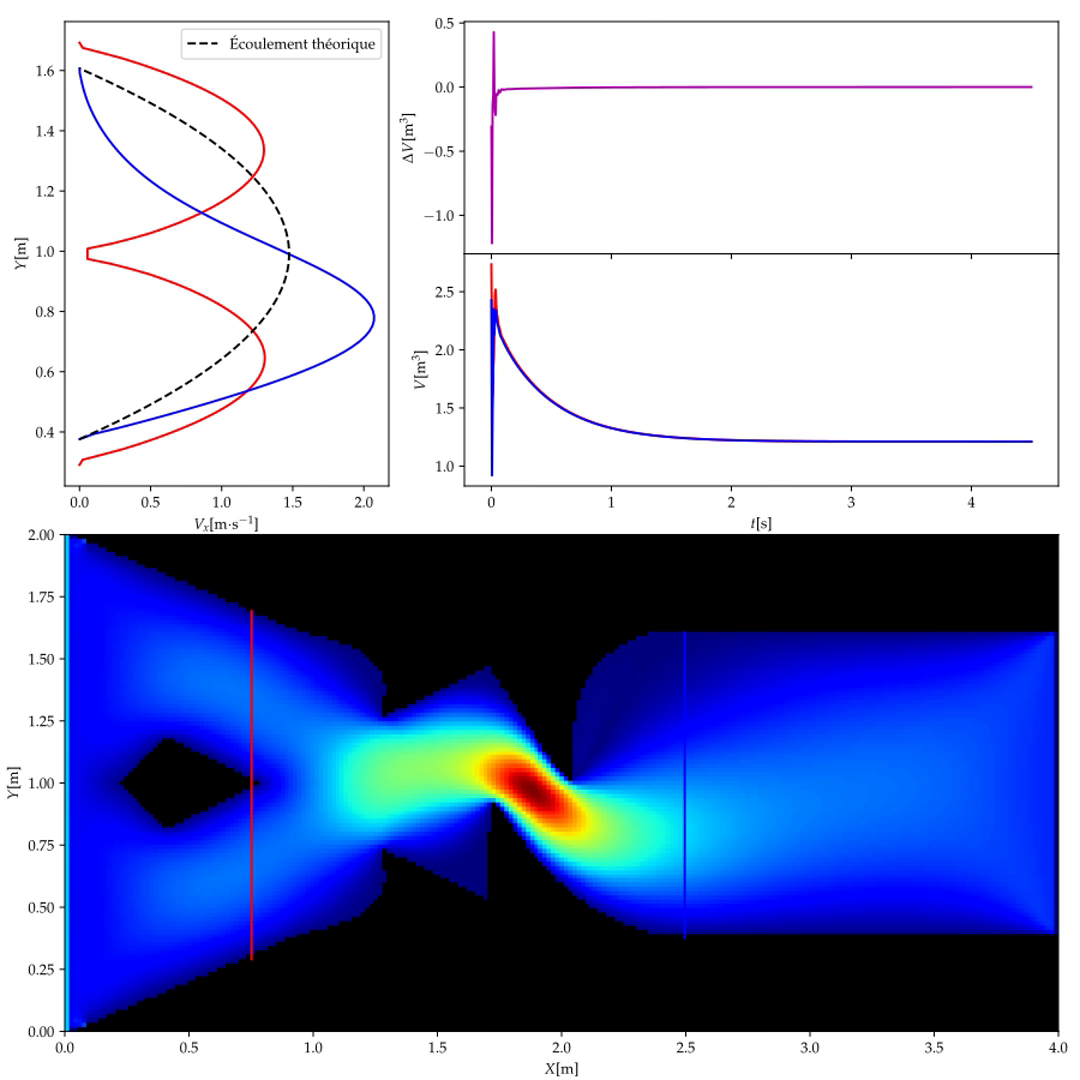
\includegraphics[width=\linewidth]{Fig/CF.png}
  \caption{Étude de l'écoulement dans une géométrie complexe}
  \label{fig:CF}
\end{figure}

La méthode lattice Boltzmann s'adapte donc bien à des géométries variées, et le débit volumique est toujours conservée.
Mais jusqu'à présent nous n'avons fait qu'étudier des flux qui converge vers des solutions indépendantes du temps.
